\documentclass{article}

\usepackage[utf8]{inputenc}
\usepackage[T1]{fontenc}
\usepackage{graphicx}

\begin{document}

\begin{flushright}
Błażej Pawluk, 279738
\end{flushright}

\title{WSI, Laboratorium, Lista 4}
\date{}
\maketitle

\section*{Zadanie 1}

\begin{figure}[h!]
	\centering
	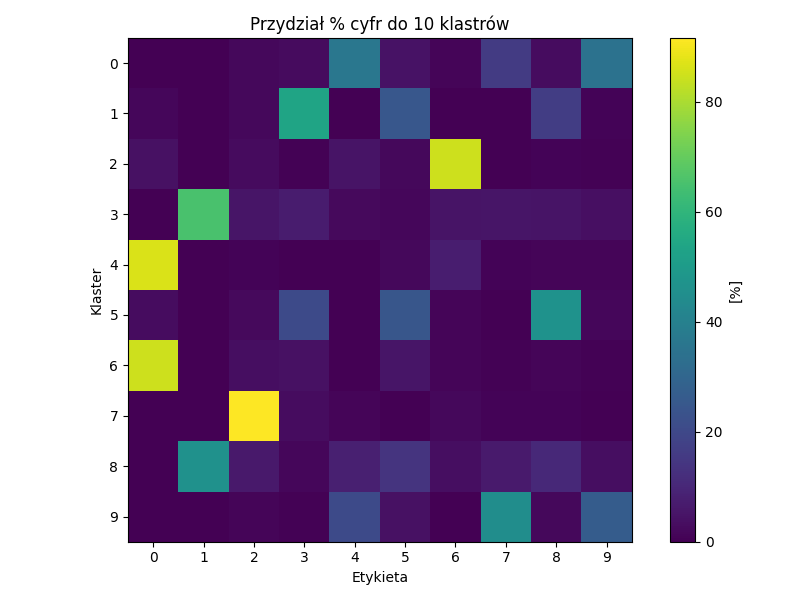
\includegraphics[width=0.5\textwidth]{images/assignment_10.png}
	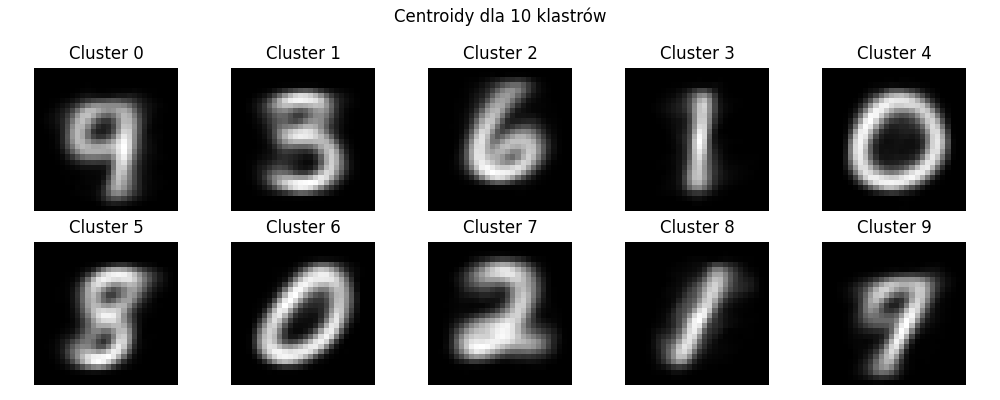
\includegraphics[width=0.5\textwidth]{images/centroids_10.png}
\end{figure}

\begin{figure}[h!]
	\centering
	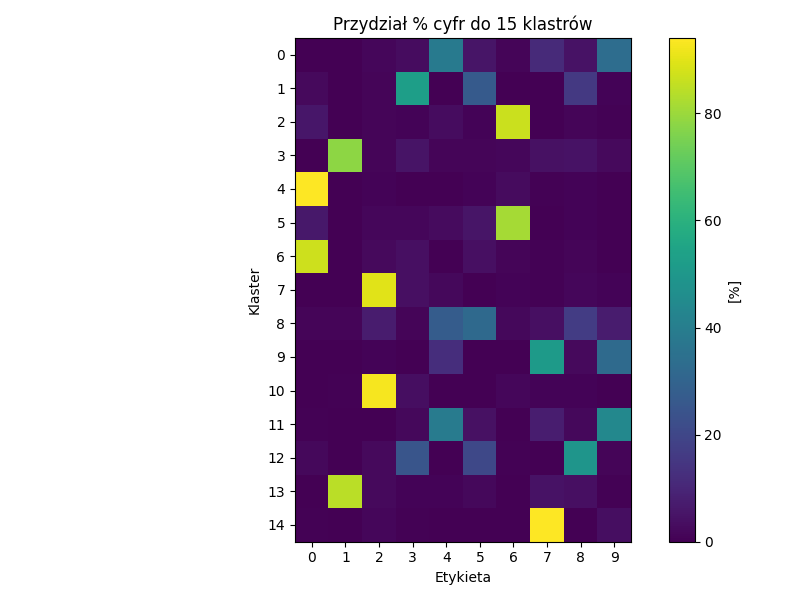
\includegraphics[width=0.5\textwidth]{images/assignment_15.png}
	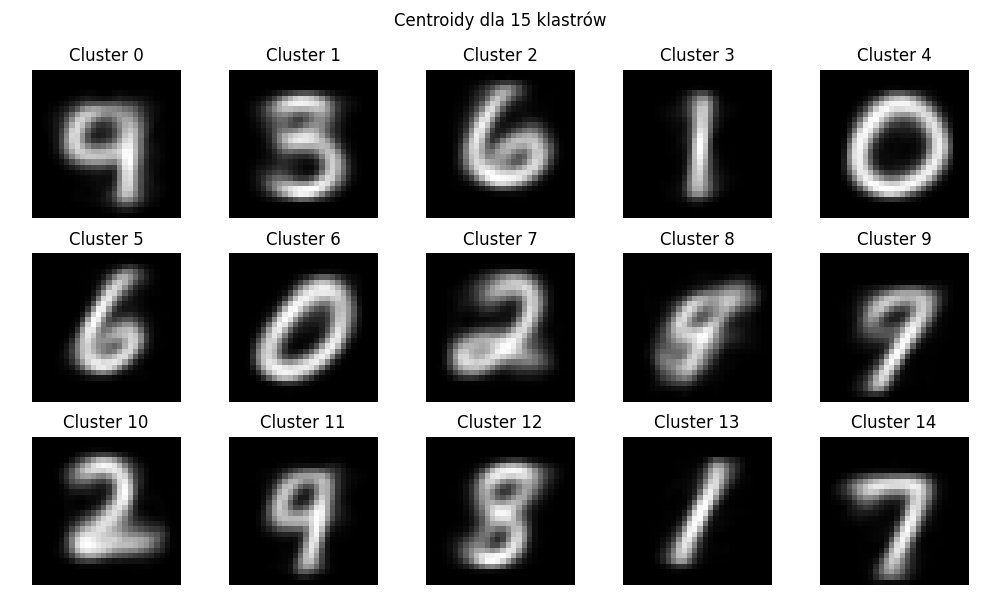
\includegraphics[width=0.5\textwidth]{images/centroids_15.png}
\end{figure}

\begin{figure}[h!]
	\centering
	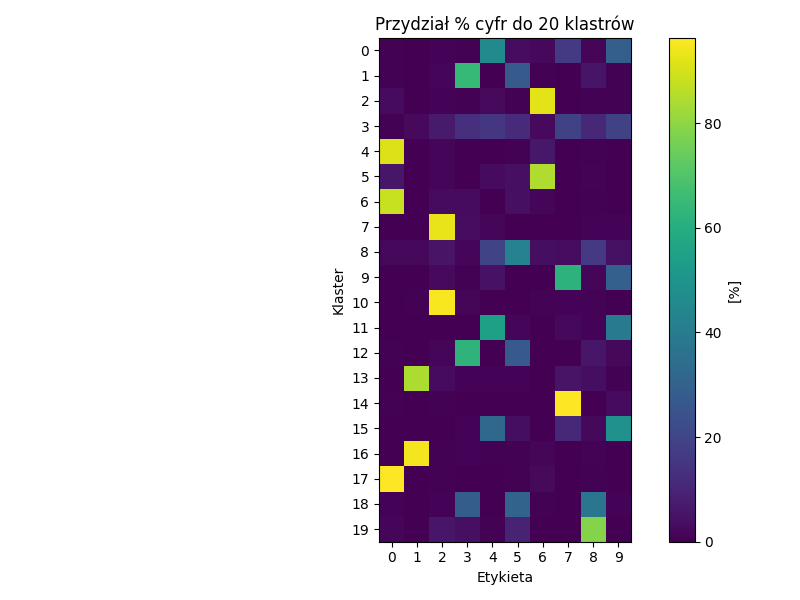
\includegraphics[width=0.5\textwidth]{images/assignment_20.png}
	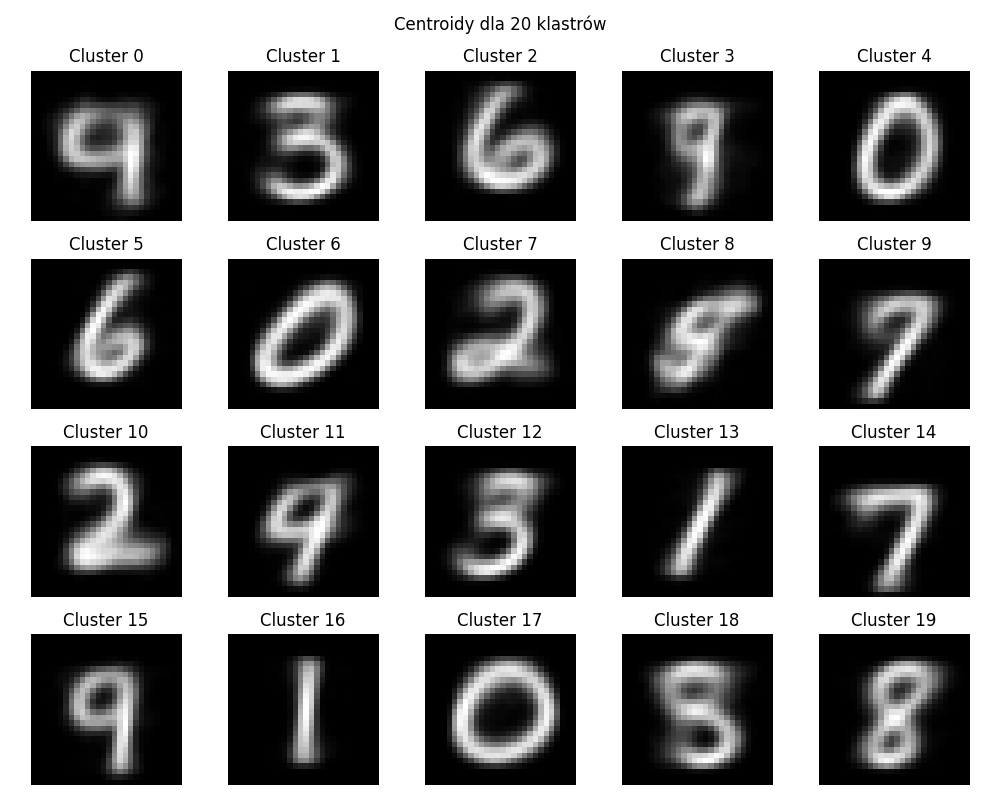
\includegraphics[width=0.5\textwidth]{images/centroids_20.png}
\end{figure}

\begin{figure}[h!]
	\centering
	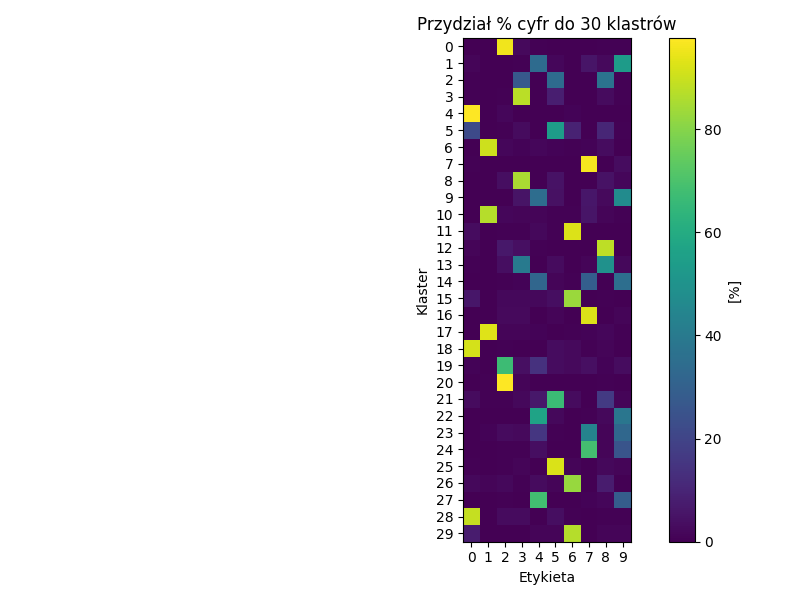
\includegraphics[width=0.5\textwidth]{images/assignment_30.png}
	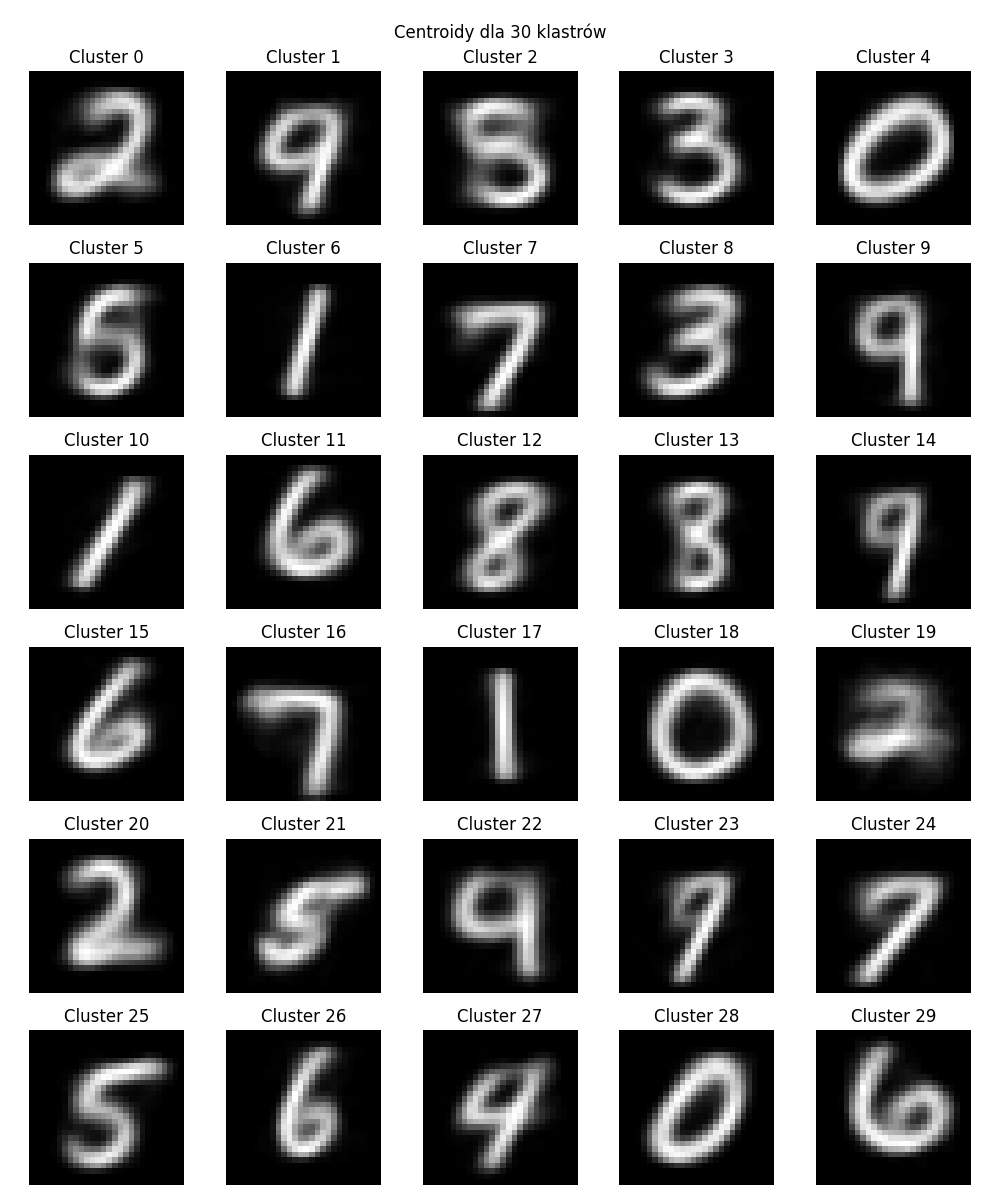
\includegraphics[width=0.5\textwidth]{images/centroids_30.png}
\end{figure}

\section*{Zadanie 2}
Wartości wejściowe:\\
	eps=0.25\\
	min_pts=5\\
\\
Statystyki:\\
	ilość klastrów=25\\
	szum=6.12\%\\
	poprawność=88.05\%\\
	błędne klasyfikacje=11.95\%\\

\begin{figure}[h!]
	\centering
	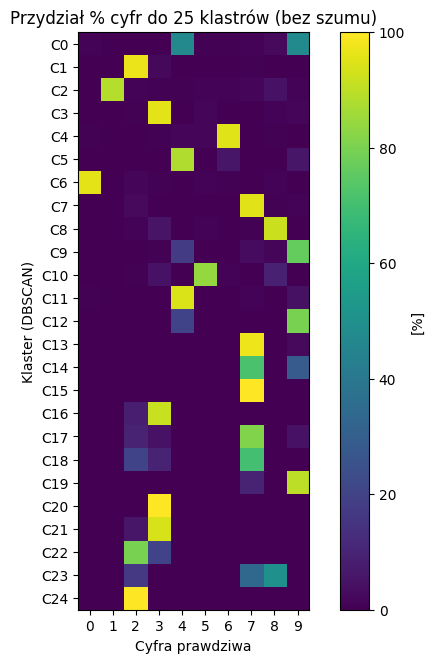
\includegraphics[width=0.5\textwidth]{images/dbscan_assignment.png}
\end{figure}

\end{document}